\documentclass{standalone}
\usepackage{pgfplots}
\begin{document}

\begin{tikzpicture}[scale=1.0]

% Continuous plot for sigma(t)
\begin{axis}[
    axis lines=middle,
    xlabel={$t$},
    ylabel={$\sigma(t)$},
    xtick=\empty,
    ytick={0,1},
    ymin=-0.5,
    ymax=1.5,
    xmin=-1,
    xmax=2,
    width=7cm,
    height=5cm,
    enlargelimits
]
% Step function
\addplot[domain=-1:0, thick] {0};
\addplot[domain=0:2, thick] {1};
\end{axis}

\end{tikzpicture}

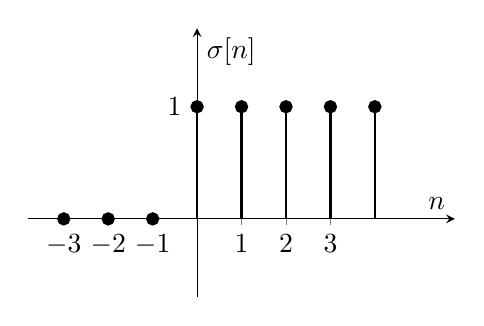
\begin{tikzpicture}[scale=1.0]

% Discrete plot for sigma[n]
\begin{axis}[
    axis lines=middle,
    xlabel={$n$},
    ylabel={$\sigma[n]$},
    xtick={-3,-2,-1,0,1,2,3},
    ytick={0,1},
    ymin=-0.5,
    ymax=1.5,
    xmin=-3,
    xmax=5,
    width=7cm,
    height=5cm,
    enlargelimits
]
% Discrete step function
\addplot[ycomb, thick, mark=*] coordinates {(-3,0) (-2,0) (-1,0) (0,1) (1,1) (2,1) (3,1) (4,1)};
\end{axis}

\end{tikzpicture}
\end{document}
